\documentclass[]{article}
\usepackage{listings}
\usepackage{hyperref}
\usepackage{graphicx}

%Commands
\newcommand{\kb}{kulturBOT}
\newcommand{\kbspace}{\kb \space}
\newcommand{\mykb}{my \kb}
\newcommand{\mykbspace}{\mykb \space}

%Code Styles
\lstdefinestyle{ssh}{
	showspaces=true,
	frame=single
}

% Title Page
\title{\kbspace Instruction Manual}
\author{Colin Gagich \\ \textnormal Version 1.0}
\date{Last Updated: \today}

\begin{document}
\maketitle

\newpage

\tableofcontents
\newpage

\section{Getting Started}
Hello there! You have been tasked with taking care of \mykb! Welcome to the team! We are glad to have you with us. Here are some things to get you started working with \kb.

\subsection{Quick Facts}

Twitter Profile: \href{https://twitter.com/kulturBOT}{@kulturBOT} \\
Facebook Profile: \href{https://www.facebook.com/thekulturbot}{Facebook Homepage}\\
Expected Battery Life: 3 Hours.\\
Expected Charge Time: 3 Hours.\\
\kbspace uses \textbf{The Futurist Manifesto} by \textit{F. T. Marinetti, 1909} to create its tweets.\\
\kb 's speech comes from the last 200 things it has tweeted.

\subsection{\mykb 's Anatomy}

\mykbspace is made from a version of the iRobot Create which is directly related to the popular in house robotic vacuum cleaner. Hidden under the front of the strainer, \kbspace has three buttons. These three buttons are used to control various functions of \kb. Refer to Figure \ref{3button} for the names of these buttons. Also take note of the names of the LED's.

	\begin{figure}[h!]
		\centering
	    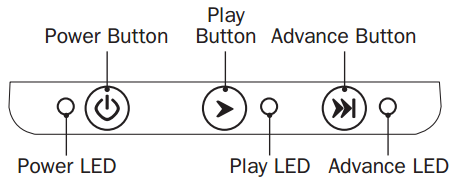
\includegraphics[width=0.8\textwidth]{img/3button.png}
	    \caption{Three Buttons Found Under Strainer}
	    \label{3button}
	\end{figure}

\subsubsection{Is \kbspace turned on?}
\label{isKbOn}
To determine if \kbspace is on, observe the \texttt{Power LED}. If it is \texttt{Green}, \kbspace is on. If it is \texttt{Orange/Amber} \kbspace is on but needs to be charged (See Section \ref{chargingKB}). If the \texttt{Power LED} is not on, \kbspace is either off or the batteries are dead.

\section{Normal Operation}
The following outlines how to get \mykbspace operating normally.

\subsection{Laptop Server and Twitter Feed}
\begin{enumerate}
	\item With the Laptop logged in, open up Visual Studio from the desktop shortcut and hit \texttt{F5}. A black Console window will open up. Refer to Figure \ref{normalVS} for an example of how it should look.
	
	\begin{figure}[h!]
		\centering
	    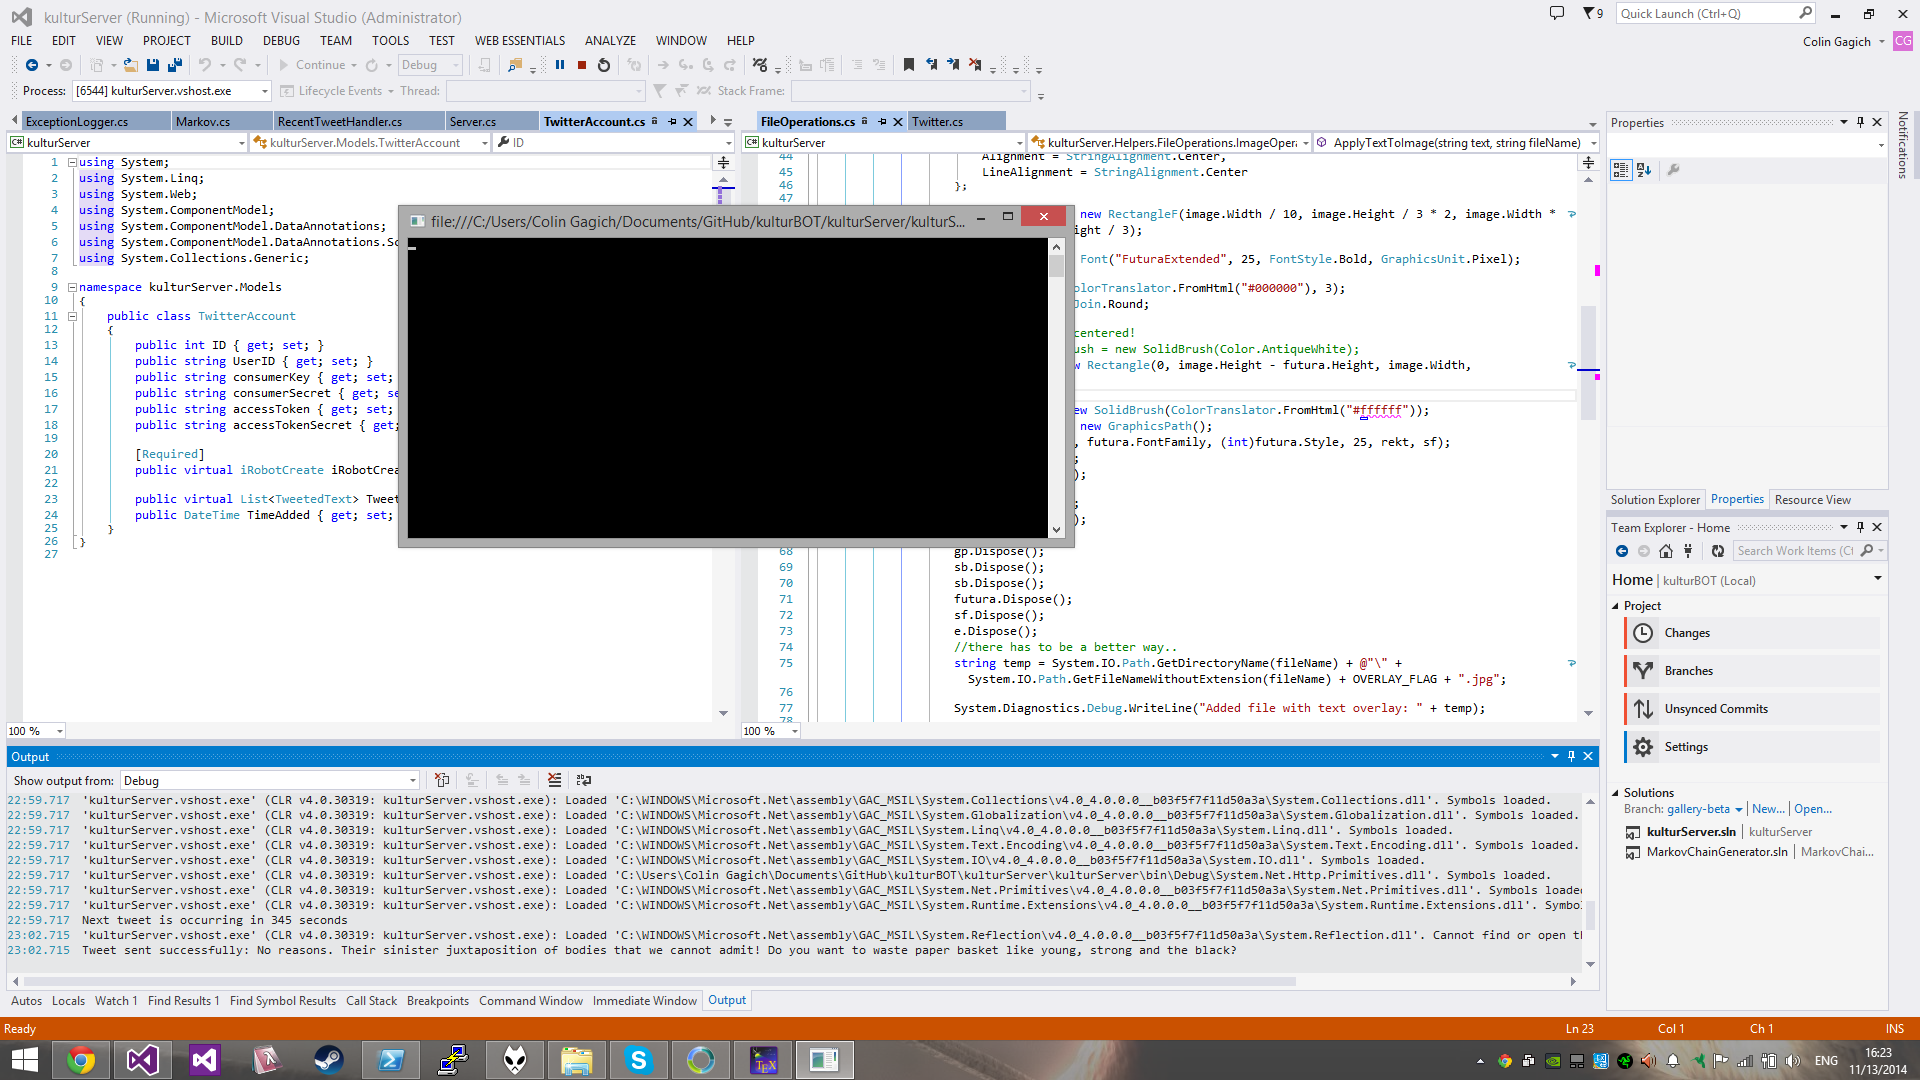
\includegraphics[width=1\textwidth]{img/normalVSlook.png}
	    \caption{Normal Operation of the Laptop}
	    \label{normalVS}
	\end{figure}
	
	\item Check the \href{https://twitter.com/kulturBOT}{\kbspace twitter feed} and ensure a tweet has been sent in the last 60 seconds. If after waiting 2 minutes no tweet appears, refer to Section \ref{kbNoTweet}. Under normal operation, no messages will appear on the black console window. If there is a problem with the internet, there will be a message in the black console window.
	
	\item To set up the live twitter feed, first connect the laptop to the projector. Ensure the projector is set up as an external display (should automatically do this). Open up Chrome from the Desktop shortcut and navigate to the \href{https://twitter.com/kulturBOT}{\kbspace twitter feed}.
	
	\item Enable the Chrome Browser Plugin "Auto Refresh Plus". Set the interval to \texttt{1 minute} and press \texttt{Start}. See Figure \ref{autorefresh} for reference.
	
	\begin{figure}[h!]
			\centering
		    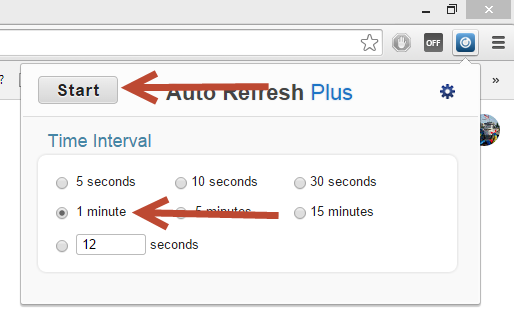
\includegraphics[width=0.55\textwidth]{img/autorefresh.png}
		    \caption{Auto Refresh Plus}
		    \label{autorefresh}
		\end{figure}
		
		\item Fullscreen the Chrome Browser by pressing \texttt{F11}.
		
		\item \textbf{NOTE:} When the Laptop turned on and the black console window is open, it will tweet \textbf{text without an image} every 2-6 minutes. This happens independently of \kbspace being turned on and functioning. Because of this, the Laptop should be shut down when the gallery is not open.
\end{enumerate}

\subsection{Connecting to the \mykbspace Unit}

\subsubsection{From a MAC or Linux Machine}

\begin{enumerate}
\item Ensure you are on the same WiFi network as \kb. In this case, kulturBOT was on the WiFi network: \texttt{Robot} with password: \texttt{Robot}
\item Open up the Terminal and enter in the following command.\\

\begin{lstlisting}[style=ssh]
ssh pi@10.20.58.151
\end{lstlisting}

\textbf{NOTICE:} The 'underscore' character represents a space.

\item You will then be prompted for a password. The password is: \texttt{raspberry} While you are typing in the password the cursor will not advance, this is a security measure.

\item You have now started an "SSH Session" with \kb. This allows you to send commands to it. To get \kbspace to move and function normally, run the following two commands, pressing enter in-between each of them.\\

\begin{lstlisting}[style=ssh]
cd kulturBOT/Test\ Client\ Server/
sudo python picam.py
\end{lstlisting}

\kbspace should \textit{beep} and then everything should function normally. The Terminal window \underline{must} remain open or kulturBOT will stop functioning.

\end{enumerate}


\subsubsection{From a Windows Machine}

Instructions coming soon.

\subsection{Stopping \mykb}

\begin{enumerate}
\item Wait until \kbspace has temporarily stopped moving. This should happen every 15-30 seconds.
\item From your Terminal Window, press \texttt{CONTROL + C}. This will end all functions on \kb.
\item To end the SSH Session with \kb, enter the following command.

\begin{lstlisting}[style=ssh]
exit
\end{lstlisting}

\end{enumerate}

If you were unable to stop \kbspace using the previous steps, try these next:

\begin{enumerate}
\item Find the \kbspace unit.
\item \textit{Aggressively} press the \texttt{Power Button} as depicted in Figure \ref{3button}.
\end{enumerate}

\subsection{Charging \mykb}
\label{chargingKB}

\begin{enumerate}
\item Determine if the \kb unit is on. Refer to Section \ref{isKbOn}
\item IF \kbspace \textbf{is on}, press the \texttt{Advance Button} one time. You should immediately hear two quick \textit{beeps}. Now press the \texttt{Play Button}. \kbspace will move on its own and find it's charging dock.
\subitem \textbf{NOTE: if you do not hear two quick beeps after pressing the \texttt{Advance Button}, restart \kb.}
\item IF \kbspace \textbf{is not on} or \textbf{wont turn on} manually pick up \kbspace and place it onto it's charging dock.
\end{enumerate}

\section{Troubleshooting}
\subsection{\kbspace isn't tweeting!}
\label{kbNoTweet}

\subsection{\kbspace is taking pictures but not moving.}
\subsection{\kbspace won't turn on.}
\end{document}          
